\documentclass{article}

\usepackage{amsmath, amsthm, amssymb, amsfonts}
\usepackage{thmtools}
\usepackage{graphicx}
\usepackage{setspace}
\usepackage{geometry}
\usepackage{float}
\usepackage{hyperref}
\usepackage[utf8]{inputenc}
\usepackage[english]{babel}
\usepackage{framed}
\usepackage[dvipsnames]{xcolor}
\usepackage{tcolorbox}

\colorlet{LightGray}{White!90!Periwinkle}
\colorlet{LightOrange}{Orange!15}
\colorlet{LightGreen}{Green!15}

\newcommand{\HRule}[1]{\rule{\linewidth}{#1}}


\setstretch{1.2}
\geometry{
    textheight=9in,
    textwidth=5.5in,
    top=1in,
    headheight=12pt,
    headsep=25pt,
    footskip=30pt
}

% ------------------------------------------------------------------------------

\begin{document}

% ------------------------------------------------------------------------------
% Cover Page and ToC
% ------------------------------------------------------------------------------

\title{ \normalsize \textsc{}
		\\ [2.0cm]
		\HRule{1.5pt} \\
		\LARGE \textbf{\uppercase{Documento di Note}
		\HRule{2.0pt} \\ [0.6cm] \LARGE{In questo documento vengono riportati i concetti affrontati durante lo stage presso Synclab S.r.L.} \vspace*{10\baselineskip}}
		}
\date{}
\author{\textbf{Author} \\ 
		Marco Brugin \\
		Synclab S.r.L. \\
		\today}

\maketitle
\newpage

\tableofcontents
\newpage

\section{Streaming ad eventi}
È una pratica di acquisizione dei dati in tempo reale da fonti di eventi come database, flussi di eventi; memorizando tutto ciò per un recupero futuro di tali informazioni, reagendo a flussi di eventi in tempo reale. Inoltre garantisce un flusso  continuo di info corrette nel posto giusto e  al momento giusto.
\subsection{Utilizzi}
\begin{itemize}
    \item per transazioni
    \item per servizzi IOT di vario genere
    \item monitoraggio sanitario 
    \item ovunque ci sia la necessità di trattare grandi moli di dati efficientemente
\end{itemize}
\section{Apache \textbf{Kafka}}
\textbf{Kafka} è una piattaforma open source che combina 3 funzionalità in modo da poter soddisfare i casi d'uso sopra citati:
\begin{itemize}
    \item pubblica e sottoscrive flussi di eventi, importandoli ed 	esportandoli da altri sistemi;
    \item archivia tali flussi in modo affidabile e duraturo;	
    \item elabora flussi di eventi in real time o in modo retrospettivo.
\end{itemize}
\subsection{Utilizzo}
\textbf{Kafka} opera su una architettura distribuita. Può essere distribuito e utilizzato in vari modi tra cui virtual machine e container, on-promise, o servizi cloud.

\subsection{Funzionamento}
\textbf{Kafka} nasce come sistema distribuito che opera su nodi che comunicano tramite protocollo \textbf{TCP} ad alte prestazioni. Data la sua natura distribuita implementa capacità di fault tollerance con rimpiazzo dei nodi guasti. 
\textbf{Kafka} è costituito da due componenti essenziali: server e client.
\subsubsection{Server}
\textbf{Kafka} viene eseguito come un cluster di uno o più server. Alcuni fanno da \textbf{broker}: livello di archiviazione. Altri assolvono il compito di \textbf{\textbf{Kafka} Connect}: importano e esportano i dati sotto forma di  flussi di eventi che permette di interagire con altri sistemi esistenti.
\subsubsection{Client}
Consentono di scrivere applicazioni distribuite e microservizi che leggono, scrivono ed elaborano flussi di eventi in parallelo, su larga scala e con fault tollerance anche in caso di problemi di rete o guasti della macchina.
Esitono molti client per diversi linguaggi di programmazione.
\subsection{Garanzie di funzionamento}
In \textbf{Kafka} esistono produttori e consumatori che producono e sottoscrivono eventi. 
Gli uni sono sono indipendenti l'uno dall'altro, ciò permette di raggiungere alcune delle seguenti garanzie:
\begin{itemize}
    \item \textbf{Al massimo una volta}: i messaggipossono andare persi ma mai riconsegnati. Infatti si potrebbe verificare un guasto ad un singolo broker o un errore della rete nel momento dell'invio di un messaggio. Il messaggio stesso verrà recapitato una e una sola volta.
    \item \textbf{Almeno una volta}: i mesaggi non 		vengono mai persi ma possono essere 		riconsegnati;
    \item \textbf{Una solo volta}: i messaggi non  		vanno persi e sono consegnati una 		sola volta; è la garanzia maggiormente desiderabile.
\end{itemize}
\subsection{Gestione degli eventi}
Gli eventi sono organizzati in topic o argomenti. Gli eventi possono essere letti da più consumatori. 
Un evento anche se consumato non viene eliminato, può essere impostato un timeout di mantenimento dell'evento.
I topic sono partizionati su più nodi. Tale partizionamento consente ai client di leggere e scrivere dati da/a molti broker. Quando un nuovo evento viene emesso questo si aggiunge all rispettiva partizione. Sarà \textbf{\textbf{Kafka}} a garantire che gli eventi vengano letti nell'ordine in cui sono stati scritti.
\subsection{Interfacce presentì}
\subsubsection{\textbf{Kafka} Producer}
L’interfaccia Producer permette alle applicazioni di inviare i flussi di dati ai broker di un cluster di Apache per categorizzarli e salvarli (nei topic già citati).
\subsubsection{\textbf{Kafka} Consumer}
L’interfaccia Consumer consente ai consumatori di Apache \textbf{Kafka} di  ricevere l’accesso ai dati, salvati nei topic di un cluster.
 \subsubsection{\textbf{Kafka} Connect}
    L’interfaccia Connect  consente di impostare produttori e consumatori riutilizzabili che collegano i topic di \textbf{Kafka} con le applicazioni o le banche dati esistenti.
\subsection{Casi d'uso}
\subsubsection{Notifica dell'evento}
\textbf{Kafka} permette di trasmette semplicemente eventi per avvisare altri sistemi di un cambiamento nel suo dominio.
\subsubsection{Trasferimento di stato portato da eventi}
In questo utilizzo il destinatario dell'evento ottiene anche i dati di cui ha bisogno per eseguire azioni aggiuntive sui dati richiesti.
\subsubsection{Approvvigionamento di eventi}
In questo caso il sistema consente di descrivere ogni cambiamento di stato in un sistema come un evento, con ogni evento registrato in sequenza cronologica. Di conseguenza, il flusso di eventi stesso diventa la principale fonte di verità del sistema.
\subsection{Applicazioni}
\subsubsection{Messaggistica}
I broker di messaggi vengono utilizzati per disaccoppiare l'elaborazione del messaggio dal produttore dello stesso.
\textbf{Kafka} rispetto ai sistemi di messaggistica tradizionale ha una migliore velocità, partizionamento integrato e tolleranza agli errori.
L'utilizzo è basso, ma in ambiti in cui si richiede una bassa latenza, le garanzie fornite da \textbf{Kafka} sono alla pari dei tradizionali sistemi di messagistica, che lo rendono lo rendono una buona soluzione per applicazioni di elaborazione di messaggi su larga scala.

\subsubsection{Monitoraggio di siti web}
È il caso d'uso d'origine di \textbf{Kafka} , ha la caratteristica di generare un elevato volume di messaggi. Lo scopo era quello di ricostruire le attività degli utenti come insieme di eventi genrati dalle azioni dell'utente.
\subsubsection{Metrica}
Indica l'aggregazione di dati di monitoraggio provenienti da varie fonti per eseguire statistiche.
\subsubsection{Aggregazione di registri}
\textbf{Kafka} ha anche la capacità di estrarre i dati dai file di log fisici e fornisce una astrazione di tali sotto forma di flusso di messaggi. Ciò permette di garantire una più bassa latenza di elaborazione e supporto per più origini dati.
\subsubsection{Elaborazione del flusso}
È possibile andare a creare una  data-pipeline in cui i dati grezzi vengono consumati dagli argomenti di \textbf{Kafka}, aggregati, trasformati fino ad ottenere unn dato elaborato.
\subsubsection{Approvvigionamento di eventi}
È possibile utilizzare  di \textbf{Kafka} in aplicazioni cui cambiamenti di stato vengono registrati come sequenze di record in ordine temporale. \textbf{Kafka} permette il supporto per dati di registro memorizzati molto grandi tanto che lo rende un ottimo back-end di tali applicazioni. 
\subsubsection{Registro commit}
\textbf{Kafka} può fungere da sorta di log di commit esterno per un sistema distribuito. Il registro aiuta a replicare i dati tra i nodi e funge da meccanismo di risincronizzazione per consentire ai nodi non allineati di ripristinare i propri dati.

\subsection{Apache Kafka VS EDA}
L'emissione di un evento indica che qualcosa è accaduto e può essere visto come un agglomerato di dati atomico in grado di soddisfare l'evento stesso. 
\textbf{Kafka} è un sistema di streaming di eventi che gestisce un flusso continuo di eventi. Inoltre Kafka memorizza tali in modo duraturo per il successivo recupero, analisi o elaborazione in tempo reale e li inoltri a varie destinazioni secondo necessità.
\\
D'altra parte in una \textbf{EDA} (Event Driven Architecture) viene generati degli eventi che un agente acquisisce e risponde a tale evento.
per utilizzare \textbf{Kafka} in un sistema \textbf{EDA} la chiave è andare a sfruttare il disaccopiamento: invece di effetuare un polling continuo di verifica della presenza di nuovi dati, basterà ascoltare il verificarsi di un evento per agire. Inoltre grazie all'approcio sviluppato da \textbf{Kafka} un evento una volta soddisfatto non viene eliminato, ma conservato per un periodo ti tempo predeterminato, pertanto un evento potrà essere letto da più consumatori e potrà essere utilizzato per soddisfare una varietà di richieste.
\section{Even Driven Architecture}
L'\textbf{Even Driven Architecture} è un pattern archietteturale basato su eventi: degli agenti, che sono in grado di ricevere tali eventi, agiranno solo nel momento in cui questi ultimi si verificheranno. 
Una architettura basato su eventi fornisce una serie di altri vantaggi basati sul disaccopiamento tra il produttore e il consumatore dell'evento, i quali, nel momento dell'emissione di quest'ultimo non è necessario siano sincroni ma possono andare a sfruttare una comunicazione di tipo asincrona. 
\subsection{Casi d'uso}
\subsection{Integrazioni esterne}
In molti sistemi quando di verifica un evento è necessario interagire con un servizio esterno. Grazie ad una architettura ad eventi, ogni servizio sarà indipendente l'uno dall'altro, così che se un servizio riscontra problemi nella sua esecuzione gli altri non ne risenteranno, data la loro indipendenza. Inoltre anche l'aggiunta di nuovi servizi ha nessun impatto. 
\subsection{Flussi di lavoro}
L'archiettetura \textbf{EDA} può essere anche impiegata nell'orchestrazione di un flusso di lavoro; nel quale ogni servizio è responsabile di un part del flusso indipendentemente dagli altri. Il fattore chiave è andare ad eseguire il rispettivo servizio all'emissione di un determinato evento.
\subsection{Trasferimento di Stato}
La modifica di un dato è un altro caso d'uso in cui l'architettura \textbf{EDA} può essere utilizzato per segnalare in tempo reale il mutamento di un dato in una detrminata struttura dati.
\subsection{Accoppiamento temporale}
Inoltre grazie ad un' architettura \textbf{EDA} si va a rimuovere l'accopiamento temporale tra chi efettua una chiamata e chi va a risponde a quest'ultima.
\section{Middleware}
Con il termine di \textbf{Middleware} si va ad intendere un insieme di pacchetti software che molte applicazioni utilizzano per comunicare tra di loro. Il \textbf{Middleware} funge da ponte tra tecnologie differenti in modo da poterle totalmente integrare.\\
L'architettura sottostante ad un \textbf{Middleware} non è altro che una \textbf{data-pipeline} nella quale i dati passano da una applicazione in connessione all'altra. \\
La chiave di utilizzo di un \textbf{Middleware} è che fornisce disaccopiamento tra i vari stadi di una \textbf{data-pipeline}.
\section{Panoramica design pattern architetturali}
\subsection{Layered-Architecture}
È un modello architetturale basato su più livelli orrizontali, in cui ciascuno svolge un compito specifico e ha detrminata responsabilità. Sebbene il pattern in sè non indichi il numero di livelli da utilizzare, è usuale creare architetture con al più quattro livelli: presentazione, business, persistenza e database.
In tale archittetura ogni livello è del tutto separato dagli altri: le modifiche apportate ad un livello non generano cambiamenti agli altri, per questo si parla di livelli isolati.
La comunicazione tra i livelli avviene in dall'alto verso il basso e in generale attraverso livelli chiusi: il passaggio delle informazione tra due o più livelli deve attraversare tutti i livelli intermedi.

\subsection{Client-server}
Nel pattern architetturale client-server ci sono due componenti essenziali: il client, che richiede un servizio o una prestazione, e il server che la fornisce. Il client espone porte di richesta, mentre il server espone porte di servizio. In tale architettura vige un tipo di collegamento Request-Response.
Uno dei principali vantaggi di tale pattern architetturale il calcolo centralizzato dei dati.
\pagebreak
\subsection{Pipe-filter}
Il modello architetturale \textbf{Pipe-Fileter} è caraterrizzato da trasformazioni successive del flusso di dati.
\\
I dati dall'origine vengono inviati dall'origine verso le porte di input del primo filtro, dove viene eseguita la prima elaborazione, quindi il prodotto dell'elaborazione viene fornito dallì'output all'input del filtro successivo e così via.
\\
Il fattore importante in tale pattern architetturale è l'ordine con cui vengono eseguiti tali filtri.
\subsection{Broker}
Il \textbf{Broker} pattern architetturale che può essere utilizzzato per sistemi software disaccopiati e distribuiti che interagiscono tramite chiamate remote.
Il pattern è formato da tre agenti:
\begin{itemize}
    \item il client: che accede a funzionalità del server inviadno ricbhieste al broker;
    \item il server che mette a disposizione del client i propri servizzi attraverso il broker;
    \item il broker: riceve le richieste dai cleint e una volta trovato il server appropiato inoltra la richiesta e trasmette il risultato al client.
\end{itemize}
\section{Publisher-Subscriber}
Il pattern architetturale \textbf{Publisher-Subscriber} è un modello di progettazione software, utilizzato nei sistemi distribuiti, che impiegano una comunicazione asincrona tra i vari componenti.\\
Sebbene vada ad utilizare tecniche già preesistenti come la sottoscrizione e l'accodamento di messaggi, la  chiave di sucesso di tale pattern è il totale disoccopiamento delle componenti: i componenti non sono a conoscenza dell'identità e della presenza degli altri.\\
Il modello Pub-SUb è nato dalla necessità del rendere i sistemi ridimensionabili in modo dinamico.
\subsection{Architettura}
Il Pub-Sub fornisce un sistema di scambio di messaggi tra editori e sottoscrittori. Lo scambio tra questi ultimi non avviene in modo diretto tra gli agenti appena illustrati, ma viene utilizzato un intermediario che raggruppa i messaggi per argomento e fornisce disaccopiamento tra le componenti.
\subsection{Vantaggi}
\begin{itemize}
    \item \textbf{Debole accopiamento tra le componenti}: che rende il sistema più flessibile e modificabile dinamicamente;
    \item \textbf{Elevata scalabilità}: non esiste limite al numero di publisher e subscriber che possano comunicare;
    \item \textbf{Utilizzo della comunicazione ascincrona ad eventi}: non necessità della sicnrona degli attori coninvolti nella comunicazione;
    \item \textbf{Indipendente dal protocollo di comunicazione}: è integrabile con qualsiasi protocollo di comunicazione e stack tecnologico.
\end{itemize}
\section{Streaming Data pipelines}
Con il termine di 
\textbf{data-pipelines} si intende un software che consente il fluire automatico di dati da un punto ad un altro del sistema.
Di solito le origini sono molteplici e generano dati ad altissima velocità.
\\
L'architettura che sta dietro a una \textbf{data-pilenes} consente di consumare, elebaorare, archiviare dati in tempo reale, man mano che vengono generati.
Tutto ciò consente analisi e reazioni più veloci ad esigenze sorte.
\\
In generale nelle pipeline dati tradizionali estraggono, trasformano e caricano i dati prima che possano essere utilizzati.
Ma data la enorme mole di dati che le \textbf{Streaming Data pipelines} sono sottoposte, tutto ciò non è possibile.
\subsection{Architettura}
Infatti per elaborare dati in streaming provenienti da sistemi come \textbf{Kafka} è necssario creare due livelli per l'elaborazione dati: 
\begin{itemize}
    \item \textbf{Archiviazione}:
    questo livello consente la memorizzazione
    dei dati, permettendo letture e scritture a basso costo in termini computazionali mantenendo l'ordine di arrivo dei dati;
    \item \textbf{Lavorazione}: elabora e consuma i dati del livello di archiviazione andando a segnalare a quest'ultimo i dati non più necessari.
\end{itemize}
\subsection{Obiettivi}
\begin{itemize}
    \item \textbf{Scalabilità}: il volume dei dati può crescere notevolmente nel tempo quindi è necessario archiviare i dati in un \textbf{data warehouse};
    \item \textbf{Durata e consistenza}: è importante considerare che i dati letti potrebbero essere già modificati o obsoleti, quindi è fondamentale disporre di strumenti di monitoraggio del flusso dati nel tempo;
    \item \textbf{Ordinare}: l'archiettura deve essere in grado di individuare la sequenza dei dati nel flusso;
    \item 
    \textbf{Tolleranza ai guasti}: lo streaming dei dati non smettono mai di fluire da varie sorgenti e il sitema deve prevenire le interuuzioni di alcuni sorgentii;
    \item 
    \textbf{Latenza}: data l'enorme mole di dati prodotti, se questi ultimi non vengono gestiti in tempo reale perdono di rillevanza e diventano inutilizzabili.
\end{itemize}
\clearpage
\subsection{Alta affidabilità}
Il concetto di alta affidabilità è essenzialmente alla capacità di un sistema di funzionare continuamente senza guasti in un detrminato periodo di tempo.\\
Per garantire tali prestazioni in generale è necessario seguire i seguenti principi:
\begin{itemize}
    \item \textbf{Crossover affidabile}: creazione di ridondanza eseguendo l atto di passare dal componente X al componente Y senza perdere dati o influire sulle prestazioni;
    \item \textbf{Bilancio del carico}:
    tecnica attraverso  la quale si va a ridristribuire
    il carico di elaborazione da su tutte le risorse del sistema in modo tale che nessuna sia sovraccaricata;
    \item \textbf{Rillevazione e gestione automatica dei guasti}:
    i guasti devono essere visibili e i  sistemi devono disporre di un sistema deve essere provvisto di un sistema automatico in grado di gestirli autonomamente.
\end{itemize}
\section{Archietture distribuite}
Con il termine \textbf{distribuito} si va ad intendere un'architettura nella quale i componenti non si trovano su un'unica macchina ma possono cooperare attraverso una rete di comunicazione per raggiungere un detrminato obiettivo.
\\Le principali caraterristiche che si riscontrano su tale archietettura sono:
\begin{itemize}
    \item l'elaborazione non è limitata a una sola macchina;
    \item Il middleware è un'infrastruttura che supporta adeguatamente lo sviluppo e l'esecuzione di applicazioni distribuite, fornendo un buffer tra le applicazioni e la rete. Svolge il ruolo di intermediario del sistema e gestisce o supporta i diversi componenti di un sistema distribuito;
    \item le basi di un'architettura distribuita sono la  trasparenza, affidabilità e disponibilità.
\end{itemize}
\subsection{Confronto Architetture centralizzate e distribuite }
\begin{figure}[H]
    \centering
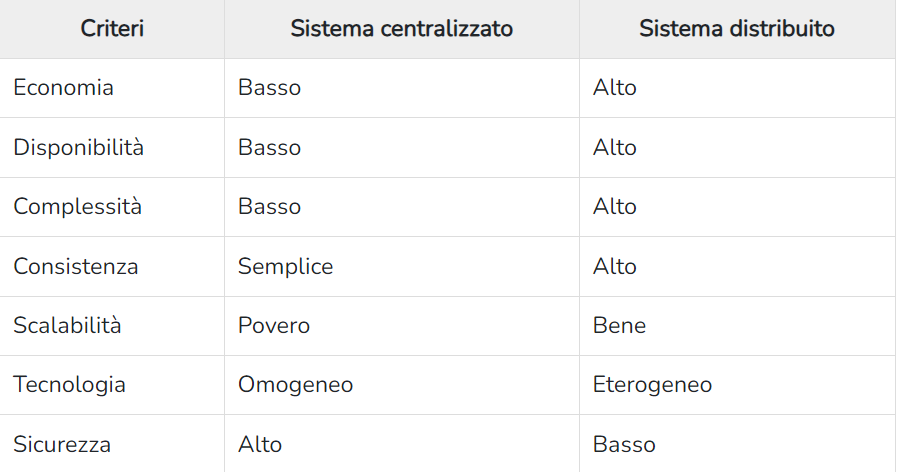
\includegraphics[scale=0.5]{images/central_vs_distribution.png}
    \caption{Confronto tra architetture centralizzate e distribuite}
    
\end{figure}
\bibliographystyle{IEEEtran}
\bibliography{https://Kafka.apache.org/documentation/}
\bibliography{https://ably.com/topic/pub-sub#the-pub-sub-model-explained}


\end{document}
